\documentclass{article}

\usepackage[english]{babel}
\usepackage{arabtex}
\usepackage{utf8}
\usepackage[utf8]{inputenc}
\usepackage{amsmath,amssymb}
\usepackage{parskip}
\usepackage{graphicx}
\usepackage{enumitem}
\usepackage{multirow}
\usepackage{tabularx}

\usepackage{hyperref}
\hypersetup{
    colorlinks,
    linkcolor={red!50!black},
    citecolor={blue!50!black},
    urlcolor={blue!80!black}
}

% Margins
\usepackage[top=2.5cm, left=3cm, right=3cm, bottom=4.0cm]{geometry}
% Colour table cells
\usepackage[table]{xcolor}

% Get larger line spacing in table
\newcommand{\tablespace}{\\[1.25mm]}
\newcommand\Tstrut{\rule{0pt}{2.6ex}}         % = `top' strut
\newcommand\tstrut{\rule{0pt}{2.0ex}}         % = `top' strut
\newcommand\Bstrut{\rule[-0.9ex]{0pt}{0pt}}   % = `bottom' strut

%%%%%%%%%%%%%%%%%
%     Title     %
%%%%%%%%%%%%%%%%%
\title{Machine Learning for NLP \\ Lab Report of Exercise 5}
\date{\today}

\begin{document}
\setcode{utf8}
\maketitle

%%%%%%%%%%%%%%%%%
%   Problem 1   %
%%%%%%%%%%%%%%%%%
\section{Part 1: NER using BERT}
\subsection{Data Set Overview}
\label{data_inspection}

In this assignment, we chose to use the German subset of the \textit{polyglot\_ner} data set. This data set was downloaded from HuggingFace.

We extract 2 differently sized training data sets. The small one contains 1'000 sentences, the big one contains 3'000 sentences. The evaluation set has 2000 sentences. Please note that the small training set is chosen to be a strict subset of the big training set in order to isolate the pure effect of an increase in training examples.

The datasets contain 4 Named Entity Recognition (NER) tags: Location (LOC), Organization (ORG), Person (PER), and Other (O). In Figure~\ref{fig:ner_tag_dist} the distribution of NER tags in the big training set (3000 sentences) is displayed.

Looking at the NER tag distribution it becomes obvious that the classes are hugely unbalanced. This is an important observation which will be further discussed in the section about model accuracy.

\begin{figure}[h!]
    \centering
    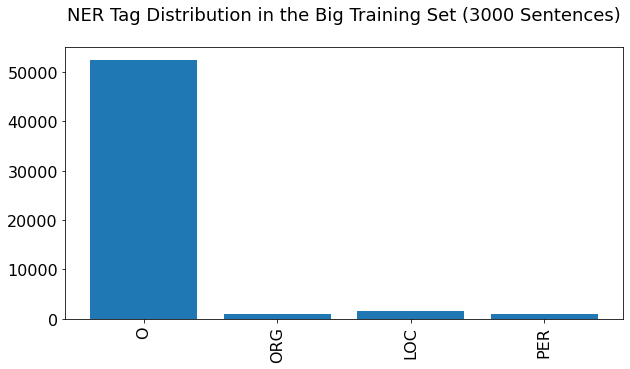
\includegraphics[scale=0.5]{ner_tag_dist.png}
    \caption{Distribution of NER Tags in the Big Training Set}
    \label{fig:ner_tag_dist}
\end{figure}


\subsection{Answers to Questions in Assignment Sheet}
In the following, the questions posed in the assignment sheet are answered:

\subsubsection{Error Message During Initialization}

According to the documentation of HuggingFace: \footnote{\url{https://huggingface.co/docs/transformers/training}}

\begin{quote}
    \textit{You will see a warning about some of the pretrained weights not being used and some weights being randomly initialized. Don’t worry, this is completely normal! The pretrained head of the BERT model is discarded, and replaced with a randomly initialized classification head. You will fine-tune this new model head on your sequence classification task, transferring the knowledge of the pretrained model to it.}
\end{quote}

\textbf{Hence, the error message arises because the head of the pre-trained BERT model is discarded and its weights randomly initialized. This is important since we want to train a new, task-specific head on top of the pre-trained model. That is also the reason why we need to specify the parameter \textit{num\_labels} when initializing a model with BertForTokenClassification.from\_pretrained(..., num\_labels=labels\_in\_our\_task).}

\subsubsection{Model Evaluation}
In Table~\ref{tab:model_eval_f1} the F1-micro and F1-macro scores of the differently fine-tuned models on the evaluation set are shown. Thereby, Small and Big Model refer to the models fine-tuned with 1'000 and 3'000 sentences, respectively.

Comparing the achieved F1-scores it becomes obvious that the \textbf{model trained on the bigger set of 3'000 sentences and frozen embeddings performs best} among the three models considered. Especially, the F1-Macro score is considerably higher for this model.

\begin{table}[h!]
\centering
\begin{tabular}{c|cc}
\multicolumn{1}{l|}{}                  & \textbf{F1-Micro} & \textbf{F1-Macro} \Tstrut\Bstrut \\ \hline
\textbf{Small Model}                   & \textit{0.932}    & \textit{0.331} \Tstrut\Bstrut    \\
\textbf{Big Model}                     & \textit{0.942}    & \textit{0.553} \Tstrut\Bstrut   \\
\textbf{Big Model (Frozen Embeddings)} & \textit{0.945}    & \textit{0.680} \Tstrut\Bstrut  
\end{tabular}
\caption{Evaluation of the 3 Models.}
\label{tab:model_eval_f1}
\end{table}

Furthermore, Figures~\ref{fig:cm_small} to ~\ref{fig:cm_bigFrozen} displays the confusion matrices for the three models on the evaluation set are shown.


\begin{figure}[]
    \centering
    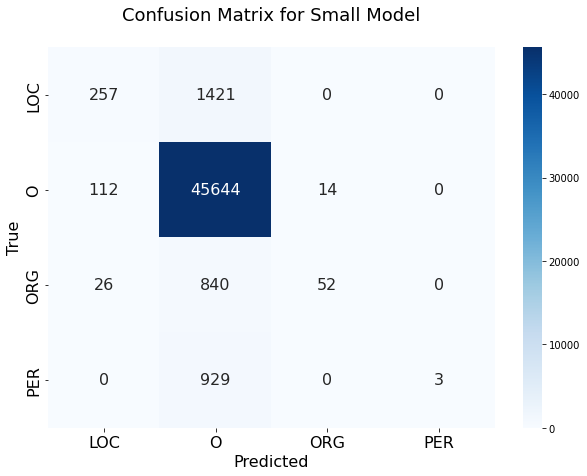
\includegraphics[scale=0.5]{confusion_matrix_smallModel.png}
    \caption{Confusion Matrix for the Small Model}
    \label{fig:cm_small}
\end{figure}

\begin{figure}[]
    \centering
    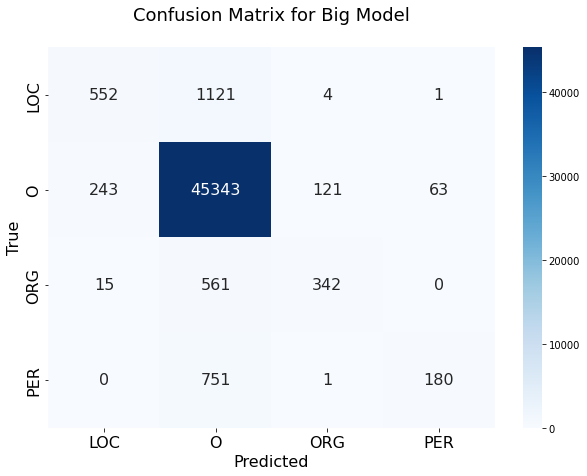
\includegraphics[scale=0.5]{confusion_matrix_bigModel.png}
    \caption{Confusion Matrix for the Big Model}
    \label{fig:cm_big}
\end{figure}

\begin{figure}[]
    \centering
    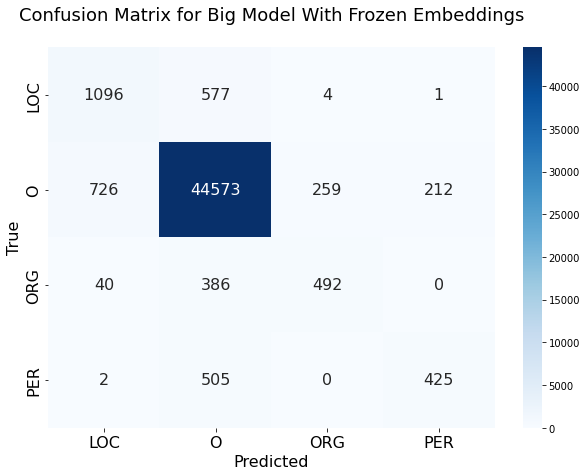
\includegraphics[scale=0.5]{confusion_matrix_bigModelFrozen.png}
    \caption{Confusion Matrix for the Big Model (Frozen Embeddings)}
    \label{fig:cm_bigFrozen}
\end{figure}


\subsubsection{Differences in F1-Micro and F1-Macro Scores}
Yes, there are significant differences in the F1-Micro and F1-Macro Scores. These differences arise due to the strong class imbalance (which was already observed in the initial data overview section).

A macro-average will compute the accuracy (of any metric, e.g., of the F1-score) independently for each class and then take the average of these individual accuracies (hence treating all classes equally). In contrast, a micro-average will aggregate the predictions of all classes and compute the metric across the entire data set (hence, giving more weight to the accuracy obtained on more frequent classes). Note that the F1-Micro average is equal to the commonly-referred 'Accuracy'.

\textbf{Hence, the differences between F1-micro and F1-macro arise if the model has a higher accuracy for certain classes than for other classes. Often, high accuracy is trivially achieved on the most frequent class by simply 'over-predicting' the most frequent class. This then yields a very high class-specific accuracy for the most frequent class, thereby pushing up the F1-Micro score while still staying at a relatively low F1-Macro score.}

Depending on the use case, either micro- or macro-averages are more important. However, whenever these two metrics are far apart, this is a strong hint of class imbalance (as is also the case in our data set). 

\subsubsection{Performance Gap Between 1'000 and 3'000 Sentences}
The performance gap between the small and big models is considerably large, especially for the F1-Macro average. Using a larger training set yields a performance improvement of 0.009 in the F1-Micro and 0.222 percentage points in the F1-Macro average, respectively.  \textbf{Consequently, our experiment suggests that it is highly advisable to use the larger training set with 3'000 sentences.}

\subsubsection{Embeddings: To freeze or not to freeze}
If the weights of the embedding layer are frozen (i.e., no weight updates are performed), an additional performance improvement of 0.003 in the F1-Micro and 0.127 percentage points in the F1-Macro averages can be achieved over the big model, respectively. \textbf{Consequently, our experiment suggests that it is better to freeze the embeddings.}

%%%%%%%%%%%%%%%%%
%   Problem 2   %
%%%%%%%%%%%%%%%%%
\pagebreak
\section{Part 2: Regression Competition}

The goal of the second task was to use the "simpletransformers" library to train a regression-type transformer model which aims to predict a metric score for the angriness of a tweet. The data contained tweets in the english language and an intensity score, indicating the intensity of the anger expressed in the tweet. 

We checked whether the "Affect Dimension" column contained only the label "anger", which was the case. We further checked in the ID column, whether the only language in the dataset was english. This was also true.

The training dataset was split into a training and a validation set. The data was split according to a 9/10 - 1/10 ratio. 

We inspected the training-, validation- and testset regarding the criterion. In order to get a good insight into how good our model performs, mean and standard deviation of all three datasets for the criterion (Intensity Score) are compared in Table \ref{tab:dfs_stats}. Fortunately, all three are comparable in means of the first two moments.

\begin{table}[h!]
    \centering
    \begin{tabular}{c|ccc}
    \multicolumn{1}{l|}{}                  & \textbf{Train} &        \textbf{Test} & \textbf{Validate} \Tstrut\Bstrut \\ \hline
    \textbf{Number of samples}                   & \textit{1531}    & \textit{1002}  & \textit{170} \Tstrut\Bstrut    \\
    \textbf{Mean}                     & \textit{0.497019}    & \textit{0.519358} & \textit{0.513547}\Tstrut\Bstrut   \\
    \textbf{Standard Deviation} & \textit{0.169095}    & \textit{0.189535} & \textit{0.175287} \Tstrut\Bstrut  
    \end{tabular}
\caption{Comparison of Basic Statistics Regarding Training and Test Set}
\label{tab:dfs_stats}
\end{table}

\subsection{Answers to Questions in Assignment Sheet}
\subsubsection{Our Experiment and Considerations on Model / Preprocessing}

For this part we chose two models, which we wanted to benchmark against each other. We hypothesized that a more generalistic model (we call it Baseline Model), not specifically trained on twitter data, would underperform an equivalent model (we call it Emotion Model), which is trained on twitter data. Both models implement the roBERTa architecture.

As can be read \href{https://huggingface.co/roberta-base}{here}, roBERTa is a transformers model pretrained on a large corpus of English data in a self-supervised fashion. This means it was pretrained on the raw texts only, with no humans labelling them in any way (which is why it can use lots of publicly available data) with an automatic process to generate inputs and labels from those texts.

More precisely, it was pretrained with the Masked language modeling (MLM) objective. Taking a sentence, the model randomly masks 15\% of the words in the input then run the entire masked sentence through the model and has to predict the masked words. This is different from traditional recurrent neural networks (RNNs) that usually see the words one after the other, or from autoregressive models like GPT which internally mask the future tokens. It allows the model to learn a bidirectional representation of the sentence.

This way, the model learns an inner representation of the English language that can then be used to extract features useful for downstream tasks: if you have a dataset of labeled sentences for instance, you can train a standard classifier using the features produced by the BERT model as inputs.

The exact names of our two models on HuggingFace.co are:
\begin{itemize}
    \item \textbf{Baseline Model:} roberta-base
    \item \textbf{Emotion Model:} cardiffnlp/twitter-roberta-base-emotion
\end{itemize}

The Baseline Model was originally trained by HuggingFace on Q\&A data and finetuned using the SQuAD2.0 dataset, the Emotion Model was trained by Cardiff NLP on around 58M tweets and finetuned for emotion recognition with the TweetEval benchmark. We choose the Baseline Model in particular because it was not trained on twitter data.

The roBERTa architecture was chosen as it is more robust than BERT. There are a few key reasons why we decided to use the roBERTa Transformer for our project. First, the roBERTa Transformer is very accurate. It has been shown to outperform other NLP models on many benchmarks. Second, the roBERTa Transformer is very fast. It can process text very quickly, which is important for us because we potentially need to be able to handle a large volume of text data (If our model is used for anger regression in a professional setting). Third, the roBERTa Transformer is very scalable. It can be easily deployed on a variety of platforms. 

Additionally we assessed whether preprocessing could help achieve better accuracy. Surprisingly we were proven otherwise: The Baseline Model achieved a pearson correlation of 0.64 on the Validation Set and the Emotion Model, achieved a correlation of 0.69. 

For preprocessing we applied the following procedure:
\begin{enumerate}
    \item we removed URLs, as they have nothing to do with how angry the person writing the tweet was.
    \item we removed \# and @ signs as they are not angriness specific.
    \item we removed punctuation. However we believe that in particular ! has some predictive power for angriness, therefore we allowed ! and ? in the tweets
    \item we removed numerals as they are not emotion-specific.
    \item we converted emojis into strings. Emojis are used by most twitter users to express emotions. They are likely a strong predictor for angriness.
    \item We believe that it is much easier for a model to deal with spell-corrected tweets. This is because the vocabulary shrinks down. For example, "hello" and "helo" are not treated the same when spelling is not corrected during preprocessing, which explodes the vocabulary. In NLP, smaller vocabulary usually means better prediction. Therefore we corrected the spelling in the tweets.
    \item we removed stopwords as they are not good predictors for angriness.
    \item we lemmatized the text. This is mainly done to shrink down the vocabulary.
    \item we lowercased the tweets, this was also done to shrink down the vocabulary. Also note that roBERTa does not include lowercasing in its preprocessing.
\end{enumerate}

Note that both the Baseline Model and the Emotion Model have automated Tokenization built-in, which is why we didn't apply it in our preprocessing pipeline.

Our results show the following:
\begin{table}[h!]
    \centering
    \begin{tabular}{c|cc}
    \multicolumn{1}{l|}{}  &   \textbf{Validation Set Baseline Model} & \textbf{Validation Set Emotion Model} \Tstrut\Bstrut \\ \hline
    \textbf{Pearson Correlation} & \textit{0.7722410084083505}    & \textit{0.8008023475420939} 
    \end{tabular}
\caption{Comparison of Pearson Correlations on the Validation Set}
\label{tab:r2s}
\end{table}

Both models performed equally well on the validation set. The estimates are however not expected to be very robust, as the sample size was very small. However, increasing the sample size for the validation set means decreasing the number of observations used during model training. It's a tradeoff between model robustness and certainty about the predictive power of the model. Keeping in mind that the training set is already very small, we decided for model robustness. It is important to be kept in mind that not much was at stake if we would obtain low accuracy on the test set. Fortunately, our decision was right, as the Emotion Model has rather good predictive power on the test set (Table \ref{tab:final_acc}).

The outcome of the direct comparison of the two models is somewhat surprising. Even though the Baseline Model was not trained on Twitter data, it still performed very well and could keep up with the Emotion Model in terms of predictive power. 
In the following we list some reasons for this model equivalence:
\begin{itemize}
    \item The data used in the study was relatively simple and both models were able to learn the patterns in the data effectively.
    \item The dataset is not extensive enough. Both models can pick up some accuracy, but with more data the differences become more and more clear.
    \item Both models have the same architecture and were trained using the same data and hyperparameters, so they had a level playing field.
    \item The Transformer models are very flexible and can be adapted to a variety of data sets, so they are likely to perform well on similar data sets.
    \item The roBERTa structure manages to incorporate a very robust representation of language.  This means that it understands language no matter what source it comes from.
    \item the transformer architecture is very robust and with enough parameters can approximate any complex relationship.
    
\end{itemize}

Due to the very slight difference in performance on the validation set, we believe that both models compare equally well! As the Emotion Model still outperforms the Baseline Model, we choose this model as our final submission. It's Pearson correlation on the test set can be found in Table \ref{tab:final_acc}. 


\subsubsection{Pearson Correlation of Best Performing Model on Testset}


\begin{table}[h!]
    \centering
    \begin{tabular}{c|cc}
    \hline
    \textbf{Pearson Correlation on Test Set} & \textit{0.7980677990705975}
    \end{tabular}
\caption{Pearson Correlation of our Best Performing Model}
\label{tab:final_acc}
\end{table}

\end{document}
